\documentclass[11pt,a4paper]{article}

\usepackage[utf8]{inputenc}
\usepackage[T1]{fontenc}
\usepackage[spanish]{babel}
\usepackage[margin=2.5cm]{geometry}
\usepackage{mathptmx}
\usepackage{enumitem}
\usepackage[colorlinks=true, linkcolor=black, urlcolor=blue, citecolor=black]{hyperref}

\renewcommand{\sectionautorefname}{Sección}
\renewcommand{\subsectionautorefname}{Sección}
\renewcommand{\tableautorefname}{Tabla}
\renewcommand{\figureautorefname}{Figura}
\usepackage{microtype}
\usepackage{graphicx}
\usepackage{booktabs}

\setlength{\parindent}{0pt}
\setlength{\parskip}{6pt}
\setlist[itemize]{leftmargin=*, itemsep=2pt, topsep=4pt}
\pagestyle{plain}

\begin{document}

\begin{center}
    {\large\bfseries PONTIFICIA UNIVERSIDAD CATÓLICA DE VALPARAÍSO}\\[0.3em]
    Facultad de Ingeniería\\[0.2em]
    Escuela de Ingeniería Informática\\[1.2em]
    {\Large\bfseries INFORME TRABAJO FINAL}\\[0.4em]
    INF3541-2 \quad TALLER DE BASE DE DATOS\\[0.8em]
    Integrantes: \textit{Agustín Guzmán y Nicolás Leiva}\\
    Fecha: \textit{noviembre de 2026}
\end{center}

\vspace{0.4em}
\hrule
\vspace{1em}

% ============================================================================
\section{Introducción}
% ============================================================================

Este informe documenta el diseño, la carga y la explotación de una base de
datos PostgreSQL construida a partir de un catálogo de películas. Se describen
el modelo, la carga mediante tablas de traspaso, los triggers de auditoría, los
procedimientos almacenados, las consultas comparadas y el control de acceso.

% ============================================================================
\section{Descripción del dataset}
% ============================================================================

\subsection{Fuente y autorización}

El dataset es un catálogo de películas compuesto por diez archivos CSV,
publicado originalmente en 2024. No cumple estrictamente el requisito de
recencia del enunciado, pero su uso fue autorizado por el profesor.

\textit{Fuente: \url{https://www.kaggle.com/datasets/gsimonx37/letterboxd}.}

\subsection{Archivos y volumen}

El conjunto ocupa aproximadamente 801 MB y contiene 941.597 películas. La
\autoref{tab:archivos} resume los archivos utilizados.

\begin{table}[htbp]
    \centering
    \begin{tabular}{l r l}
        \hline
        Archivo & Filas & Contenido \\
        \hline
        \texttt{movies.csv}    &   941.597 & Películas \\
        \texttt{posters.csv}   &   941.597 & Enlaces de póster \\
        \texttt{actors.csv}    & 5.798.450 & Reparto \\
        \texttt{crew.csv}      & 4.720.183 & Equipo técnico \\
        \texttt{studios.csv}   &   679.283 & Estudios \\
        \texttt{releases.csv}  & 1.332.782 & Estrenos por país y fecha \\
        \texttt{languages.csv} & 1.038.762 & Idiomas \\
        \texttt{countries.csv} &   693.476 & Países por película \\
        \texttt{genres.csv}    & 1.046.849 & Géneros por película \\
        \texttt{themes.csv}    &   125.641 & Temas por película \\
        \hline
    \end{tabular}
    \caption{Archivos del dataset y cantidad de filas.}
    \label{tab:archivos}
\end{table}

% ============================================================================
\section{Modelo de datos}
% ============================================================================

\subsection{Diagrama entidad-relación}

El modelo tiene 19 tablas y está en tercera forma normal. La \autoref{fig:er}
muestra el diagrama.

\begin{figure}[htbp]
    \centering
    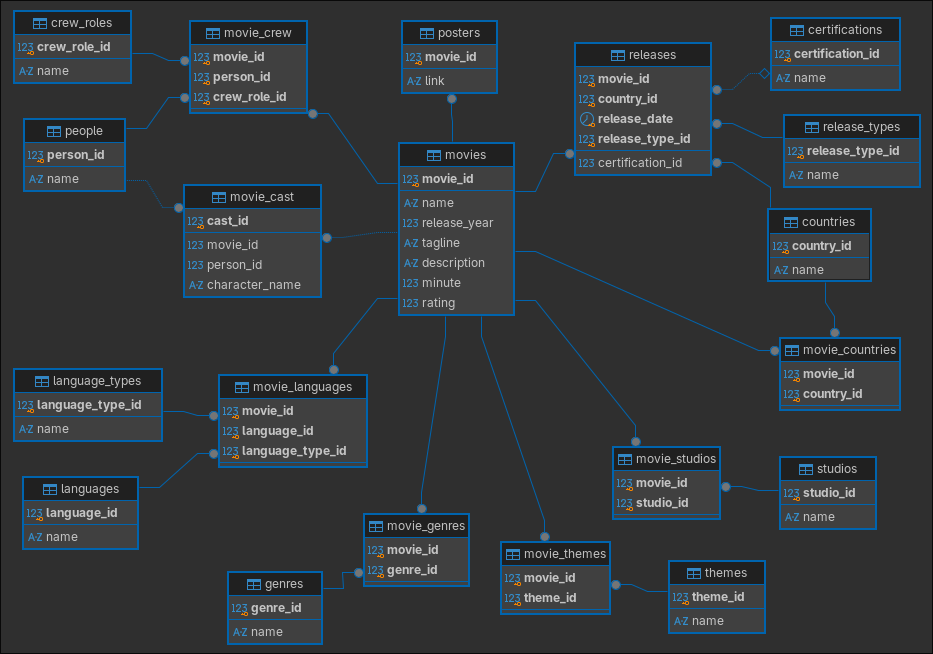
\includegraphics[width=\textwidth]{../extra/db.png}
    \caption{Diagrama entidad-relación del modelo.}
    \label{fig:er}
\end{figure}

% ============================================================================
\section{Integridad y reglas de negocio}
% ============================================================================

El esquema usa claves primarias, claves foráneas, restricciones de unicidad y
restricciones \texttt{CHECK}. Las principales validan nombre no vacío, año entre
1870 y 2100, duración positiva, rating entre 0 y 5, fechas entre 1870 y 2100 y
póster nulo o no vacío.

Las claves foráneas de las relaciones usan \texttt{ON DELETE CASCADE} hacia
\texttt{movies}. Las claves hacia catálogos y personas impiden borrar un
registro que esté en uso. Las reglas que involucran varias tablas se controlan
en los procedimientos almacenados.

% ============================================================================
\section{Carga de datos}
% ============================================================================

Los CSV se copian con \texttt{\textbackslash copy} a tablas \texttt{UNLOGGED}
del schema \texttt{staging}, sin claves foráneas ni restricciones. Luego los
scripts de \texttt{load} traspasan los datos con, aplicando \texttt{CAST},
\texttt{NULLIF}, \texttt{DISTINCT} y \texttt{JOIN} para resolver los catálogos
por nombre.

% ============================================================================
\section{Triggers de auditoría}
% ============================================================================

La tabla \texttt{audit\_log} registra la tabla afectada, la operación
(\texttt{I}, \texttt{U} o \texttt{D}), la clave de la fila, los datos anteriores
y nuevos en \texttt{JSONB}, el usuario y la fecha. Una función genérica es
reutilizada por cuatro triggers \texttt{AFTER INSERT OR UPDATE OR DELETE} sobre
\texttt{movies}, \texttt{people}, \texttt{studios} y \texttt{releases}.

Los triggers se crean después de la carga para no registrar las inserciones
masivas. Una prueba de alta, modificación y baja deja este log:

\begin{verbatim}
 operation | row_key
-----------+-------------------------
 I         | {"movie_id": 999999999}
 U         | {"movie_id": 999999999}
 D         | {"movie_id": 999999999}
\end{verbatim}

% ============================================================================
\section{Procedimientos almacenados}
% ============================================================================

Se implementaron cinco procedimientos para los mantenedores:

\begin{table}[htbp]
    \centering
    \begin{tabular}{p{4.3cm} p{9.5cm}}
        \hline
        Procedimiento & comportamiento \\
        \hline
        \texttt{sp\_movie\_upsert} &
        Exige nombre no vacío, año entre 1870 y 2100,
        duración positiva y rating entre 0 y 5. \\
        \texttt{sp\_movie\_delete} &
        Eliminación de una película. Las relaciones se eliminan por
        \texttt{ON DELETE CASCADE}. \\
        \texttt{sp\_studio\_delete} &
        No permite eliminar un estudio con películas asociadas. \\
        \texttt{sp\_person\_merge} &
        Fusiona dos personas: mueve reparto y crew y elimina el duplicado. \\
        \texttt{sp\_register\_release} &
        Registra un estreno. La fecha no puede ser anterior al año de la
        película y crea los catálogos que falten. \\
        \hline
    \end{tabular}
    \caption{Procedimientos almacenados y sus reglas de negocio.}
    \label{tab:procedimientos}
\end{table}

Todos validan sus datos y terminan con \texttt{COMMIT}. Si se incumple una regla
de negocio hacen \texttt{ROLLBACK} y lanzan una excepción; por ejemplo,
\texttt{sp\_studio\_delete} rechaza el borrado si el estudio tiene películas.
Los procedimientos no usan \texttt{SECURITY DEFINER}, porque PostgreSQL no
permite \texttt{COMMIT} ni \texttt{ROLLBACK} en ellos; por eso el rol
\texttt{bd\_mantenedor} tiene permisos \texttt{DML} sobre las tablas que
mantiene.

% ============================================================================
\section{Consultas y optimización}
% ============================================================================

\subsection{Consultas equivalentes}

La consulta A obtiene películas de Drama o Comedia, estrenadas en Estados
Unidos entre 2000 y 2009, con rating mayor o igual a 4.0. Usa enlace por
\texttt{WHERE}, \texttt{OR} e \texttt{IN}, sin \texttt{JOIN}. La consulta B
devuelve los mismos resultados con \texttt{JOIN}, una CTE y \texttt{EXISTS}.
La equivalencia se comprobó con \texttt{EXCEPT} en ambas direcciones: 0
diferencias.

\subsection{Planes antes de la optimización}

[COMPLETAR: planes antes]

\subsection{Índices creados}

Se crearon índices compuestos para buscar por género y
por país, y un índice que cubre año y rating:

\begin{verbatim}
CREATE INDEX idx_movie_genres_genre_movie
    ON movie_genres (genre_id, movie_id);

CREATE INDEX idx_movie_countries_country_movie
    ON movie_countries (country_id, movie_id);

CREATE INDEX idx_movies_year_rating
    ON movies (release_year, rating) INCLUDE (movie_id, name);
\end{verbatim}

Los índices de una sola columna quedaron cubiertos por el prefijo de los nuevos
y se eliminaron.

\subsection{Planes después de la optimización}

[COMPLETAR: planes después]

\subsection{Conclusión de la optimización}

[COMPLETAR: comparación de tiempos y conclusión]

% ============================================================================
\section{Usuarios y vistas}
% ============================================================================

Se crearon cinco vistas con filtros: \texttt{vw\_movies\_public} oculta
descripción y póster; \texttt{vw\_movies\_recent} muestra solo películas desde
2000; \texttt{vw\_releases\_public} muestra solo estrenos ya ocurridos;
\texttt{vw\_releases\_upcoming} reserva los estrenos futuros; y
\texttt{vw\_movie\_cast\_public} muestra el reparto con nombres legibles.

La \autoref{tab:roles} resume los niveles de acceso.

\begin{table}[htbp]
    \centering
    \begin{tabular}{l p{9.5cm}}
        \hline
        Rol & Acceso \\
        \hline
        \texttt{bd\_lectura} &
        Solo las vistas públicas. No puede leer las tablas base. \\
        \texttt{bd\_mantenedor} &
        \texttt{SELECT}, \texttt{DML} sobre las tablas mantenidas y ejecución de
        los procedimientos. \\
        \texttt{bd\_admin} &
        Control total del esquema, tablas, secuencias, procedimientos y
        \texttt{audit\_log}. \\
        \hline
    \end{tabular}
    \caption{Roles y niveles de acceso.}
    \label{tab:roles}
\end{table}

Con \texttt{SET ROLE} se comprobó que cada rol accede solo a lo permitido y que
\texttt{audit\_log} rechaza \texttt{UPDATE} y \texttt{TRUNCATE}.

% ============================================================================
\section{Conclusiones}
% ============================================================================

\begin{itemize}
    \item La carga en dos capas permitió separar los datos crudos de las
    transformaciones y validar los conteos al final.
    \item El modelo de 19 tablas evita redundancia y mantiene la integridad
    mediante claves y restricciones.
    \item La comparación de planes permite justificar los índices creados y su
    efecto en las consultas.
    \item Los roles y las vistas permiten exponer el catálogo sin dar acceso
    directo a las tablas base.
\end{itemize}

\end{document}
